\documentclass[../main.tex]{subfiles}

\graphicspath{{../image/}{../figure/}}

\begin{document}

\chapter{图神经网络}\label{chapter:ch13-图神经网络}

在前几章中，我们学习了以序列和图像形式出现的结构化数据，分别对应于用一维数组和二维数组存储的变量。在更广泛的应用中，有许多类型的结构化数据更适合通过图来描述，如\cref{figure:ch13-图结构化数据}所示。通常，一个图由一组称为节点的对象组成，它们通过边来连接。节点和边都可以与数据相关联。例如，在一个分子中，节点和边分别对应于不同原子类型（碳原子、氮原子、氢原子等）和不同化学键类型（单键、双键等）的离散变量相关联。对于铁路网络，每条铁路线可能与两个城市间平均旅行时间的连续变量相关联。这里我们假设边是对称的，例如从伦敦到剑桥的旅行时间与从剑桥到伦敦的旅行时间相同。这样的边可以表示为节点之间的无向连接。对于万维网而言，边是有向的，因为页面 A 上有指向页面 B 的超链接，并不一定意味着页面 B 上有指向页面 A 的超链接。

其他图结构化数据的例子有：蛋白质相互作用网络，其中节点是蛋白质，边表示蛋白质对之间相互作用的强度；电路图，其中节点是组件，边是导线；社交网络，其中节点是人，边是“友谊”。此外，还有可能存在更复杂的图结构，例如公司内部的知识图谱包含多种不同类型的节点（如人员、文档和会议），以及多种类型的边用于描述不同的属性（如一个人出席会议或一个文档引用另一个文档）。

在本章中，我们将探索如何将深度学习应用于图结构化数据。在讨论图像时，我们已经遇到了结构化数据的一个例子。在图像中，数据向量 $\bm{x}$ 的单个元素对应于规则网格上的像素。因此，图像是图结构化数据的特殊实例，其中节点是像素，边描述了哪些像素是相邻的。卷积神经网络（CNN）考虑了这种结构（参见\cref{chapter:ch10-卷积网络}），并纳入了像素之间相对位置的先验知识及一些保持属性的等变性操作（如分割），以及保持属性的不变性的操作（如分类）。我们将以图像的卷积神经网络作为启发，构建更通用的称为图神经网络的深度学习方法（Zhou et al., 2018; Wu et al., 2019; Hamilton, 2020; Veličković, 2023）。我们将看到，把深度学习应用于图结构化数据时的一个关键思路是确保对图中节点重新排序的等变性或不变性。

\begin{figure}[htbp]
  \centering
  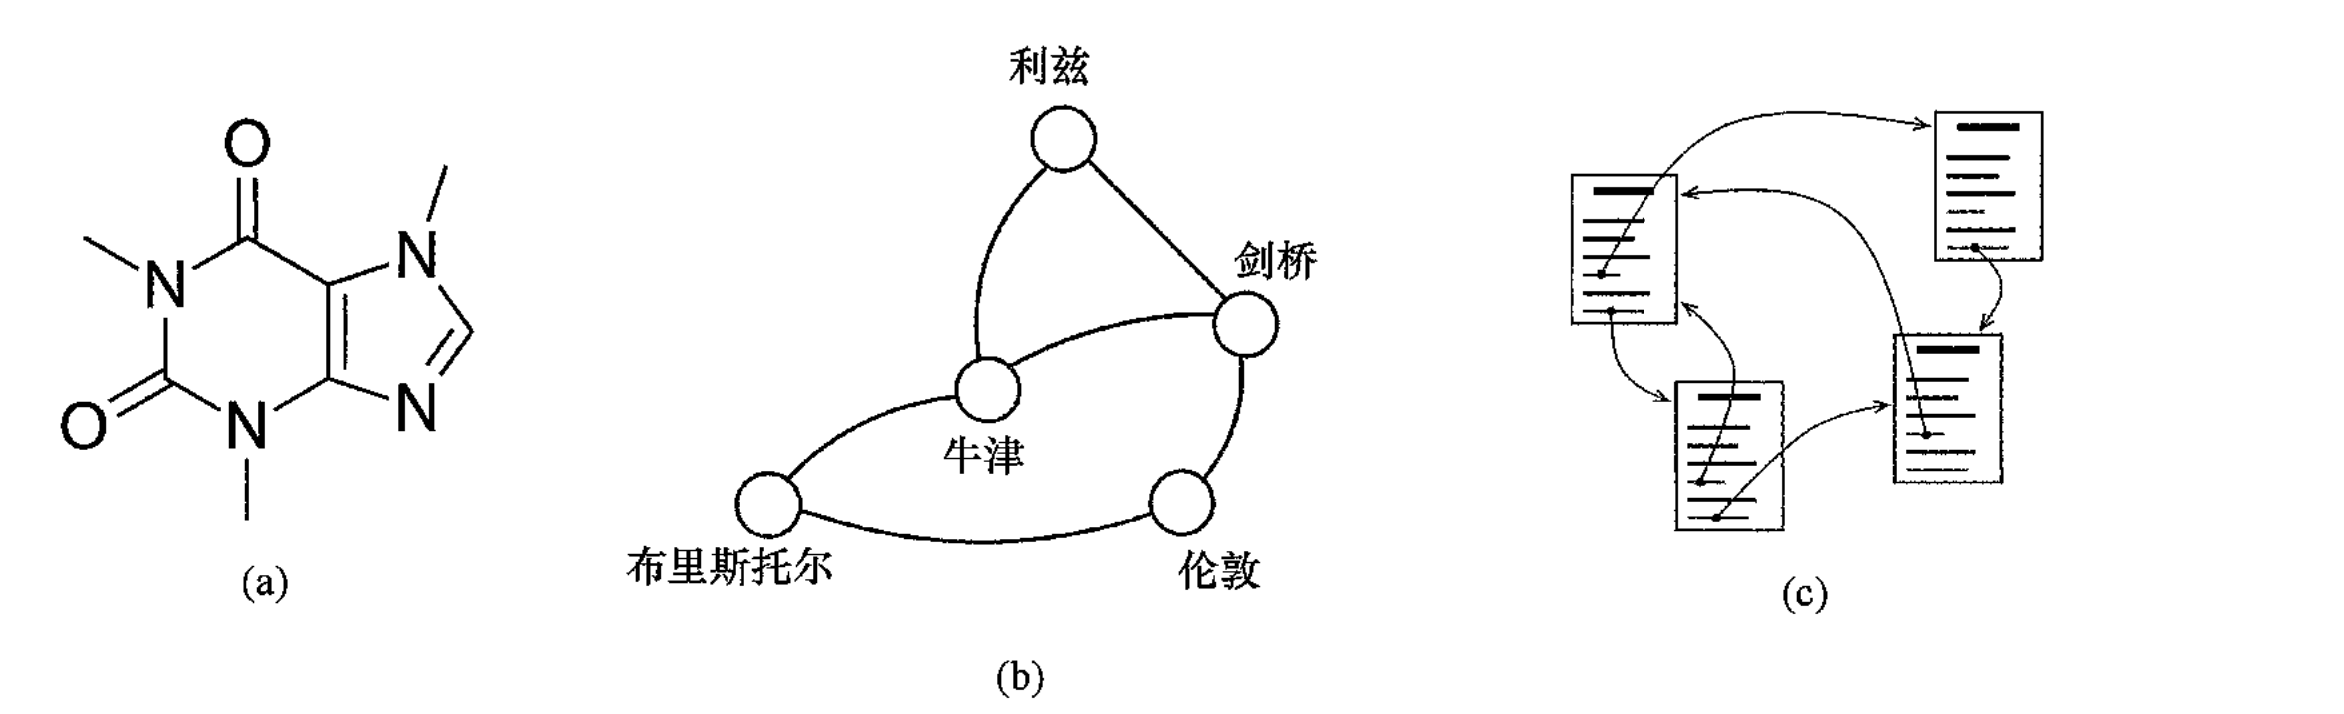
\includegraphics[width=0.95\textwidth]{ch13-fig13.1-graph-data.png}
  \caption{图结构化数据的 3 个例子：(a) 咖啡因分子由化学键连接的原子组成；(b) 由铁路线连接的城市构成的铁路网络；(c) 由超链接连接的页面构成的万维网}
  \label{figure:ch13-图结构化数据}
\end{figure}

\subfile{Chapter-13/section-01.tex}
\subfile{Chapter-13/section-02.tex}
\subfile{Chapter-13/section-03.tex}
\subfile{Chapter-13/section-04.tex}
\subfile{Chapter-13/section-05.tex}

\end{document}
